\documentclass[11pt,a4paper]{article}
\usepackage[text={6.5in,10in},centering,a4paper]{geometry}
\usepackage{indentfirst}
\usepackage{setspace}
\usepackage{amssymb,amsmath} % Equations
\usepackage{tabularx} % Tables
\usepackage{graphicx,color} % Graphics, Figures
\usepackage[tight,footnotesize]{subfigure}
\usepackage{pgfgantt} % for gantt chart
\usepackage{hyperref}
\usepackage[nottoc,numbib]{tocbibind}
\usepackage[numbers]{natbib}

\graphicspath{{figures/}} % create a director 'figures' in your local dir and all pics are kept here

\renewcommand\familydefault{\sfdefault} % set to San Serif series

\begin{document}
\thispagestyle{empty}
\begin{center}
\doublespacing
{\Large \bf Senior Project Proposal 2102490}
\vfill
{
\Large \bf
% Project title
Solar Irradiance Forecasting for Chulalongkorn University Location Using Time Series Models
}
\vfill
{\Large \bf Justin Bieber Student ID XXXX} \\[2ex]
{\Large \bf Advisor: Assist. Prof. Jitkomut Songsiri}
\vfill
{\Large \bf Department of Electrical Engineering, Faculty of Engineering} \\[2ex]
{\Large \bf Chulalongkorn University} \\[2ex]
{\Large \bf Academic Year 20XX}
\end{center}

\newpage
\thispagestyle{empty}
\tableofcontents

\newpage
\setcounter{page}{1}
\section{Introduction}

\subsection{Motivation}

\subsection{Objectives}

\subsection{Scope of work}

\subsection{Expected outcomes}

\section{Methodology}

\section{Preliminary results}

\section{Conclusions}

\subsection{Summary}

\subsection{Project plans}

\begin{figure}[h]
\noindent\resizebox{0.9\textwidth}{!}{
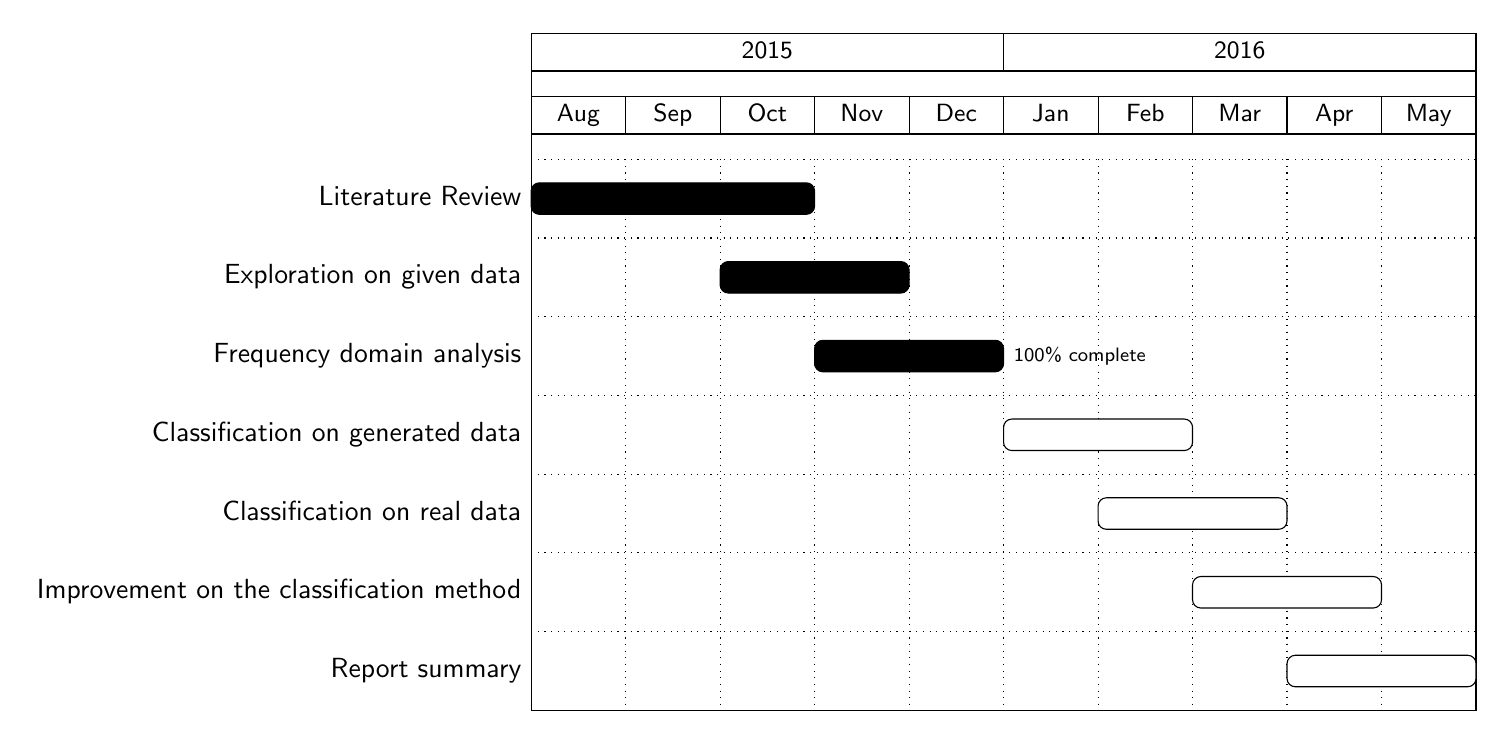
\begin{tikzpicture}
\begin{ganttchart}[
hgrid,
vgrid,
x unit = 1.2cm,
y unit title= 0.8cm,
bar/.append style={rounded corners=3pt},
time slot format=isodate-yearmonth,
time slot unit=month
]{2015-08}{2016-05}
\gantttitlecalendar{year, month=shortname}\\
\ganttbar[
bar/.append style={fill=black, rounded corners=3pt}
]{Literature Review}{2015-08}{2015-10} \\
\ganttbar[
bar/.append style={fill=black, rounded corners=3pt}
]{Exploration on given data}{2015-10}{2015-11}\\
\ganttbar[
bar/.append style={fill=black, rounded corners=3pt},
progress=100]{Frequency domain analysis}{2015-11}{2015-12}\\
\ganttbar{Classification on generated data}{2016-01}{2016-02}\\
\ganttbar{Classification on real data}{2016-02}{2016-03}\\
\ganttbar{Improvement on the classification method}{2016-03}{2016-04}\\
\ganttbar{Report summary}{2016-04}{2016-05}
\end{ganttchart}
\end{tikzpicture}
}
\caption{\label{fig:gantt} Gantt chart of the project}
\end{figure}

\subsection{Problems and solutions}

\section{List of LaTeX usage}

\subsection{Tables}
\begin{table}[ht]
\centering
\caption{Example} 
\vspace{3mm}
\begin{tabular}{|l|c|c|r|} \hline
Item & Font & Font Type & Font Size \\ \hline
Title & Garamond & Bold & 20 \\
Author names & Garamond & Bold & 12 \\ 
Author affiliation/email & Garamond & Regular & 11 \\
Abstract/Keywords & Garamond & Regular & 11 \\
Level 1 headings & Garamond & Bold & 12 \\
Level 2 headings & Garamond & Bold & 11 \\
Level 3 headings & Garamond & Regular & 11 \\
Figure/table captions & Garamond & Regular & 11 \\
Main text/References & Garamond & Regular & 11 \\ \hline
\end{tabular}
\end{table}

\subsection{Figures}

\begin{figure}[ht]
	\begin{center}
		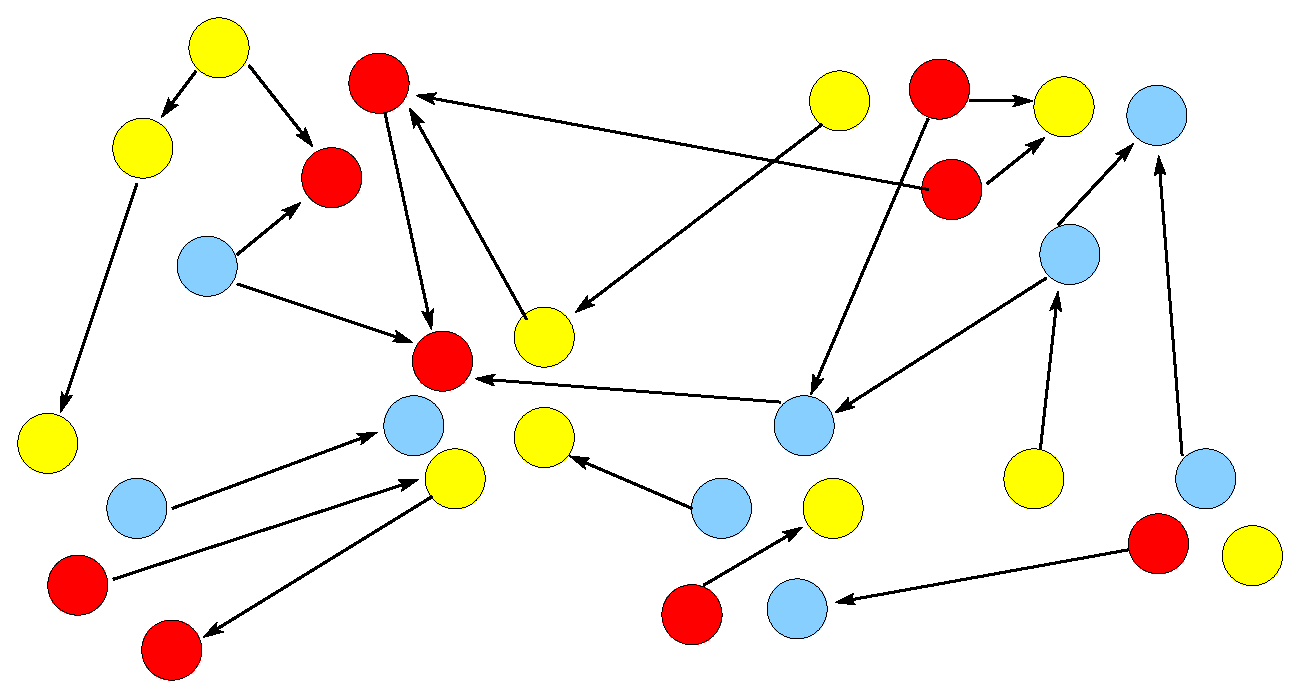
\includegraphics[width=0.7\linewidth]{gm.eps}
		\caption{Graphical model}
	\end{center}
\end{figure}

\begin{figure}[h!]
	\begin{center}
		\includegraphics[width=0.5\linewidth]{brain.jpg}
		\caption{Brain impulses (Source: Shutterstock.com Image by: Alex Mit)}
	\end{center}
\end{figure}

\begin{figure}
\centering
\subfigure[first caption]{ 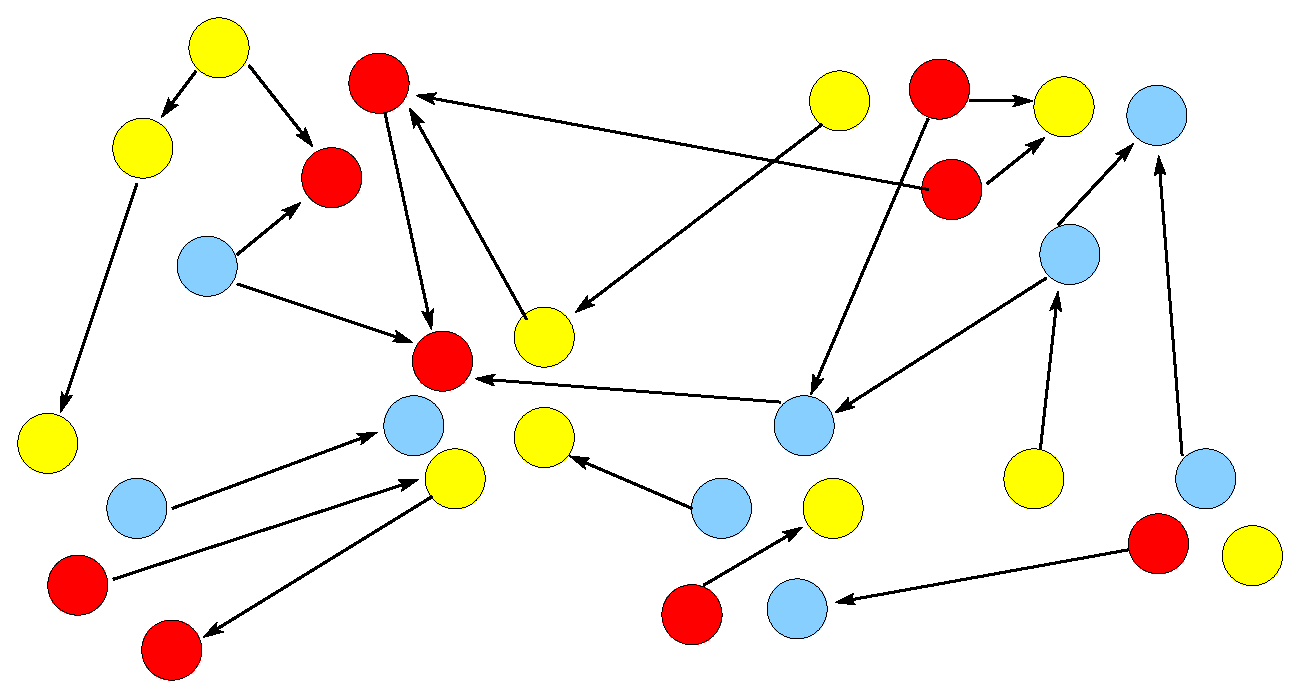
\includegraphics[width=0.45\linewidth]{gm.eps}  } 
\subfigure[second caption]{ 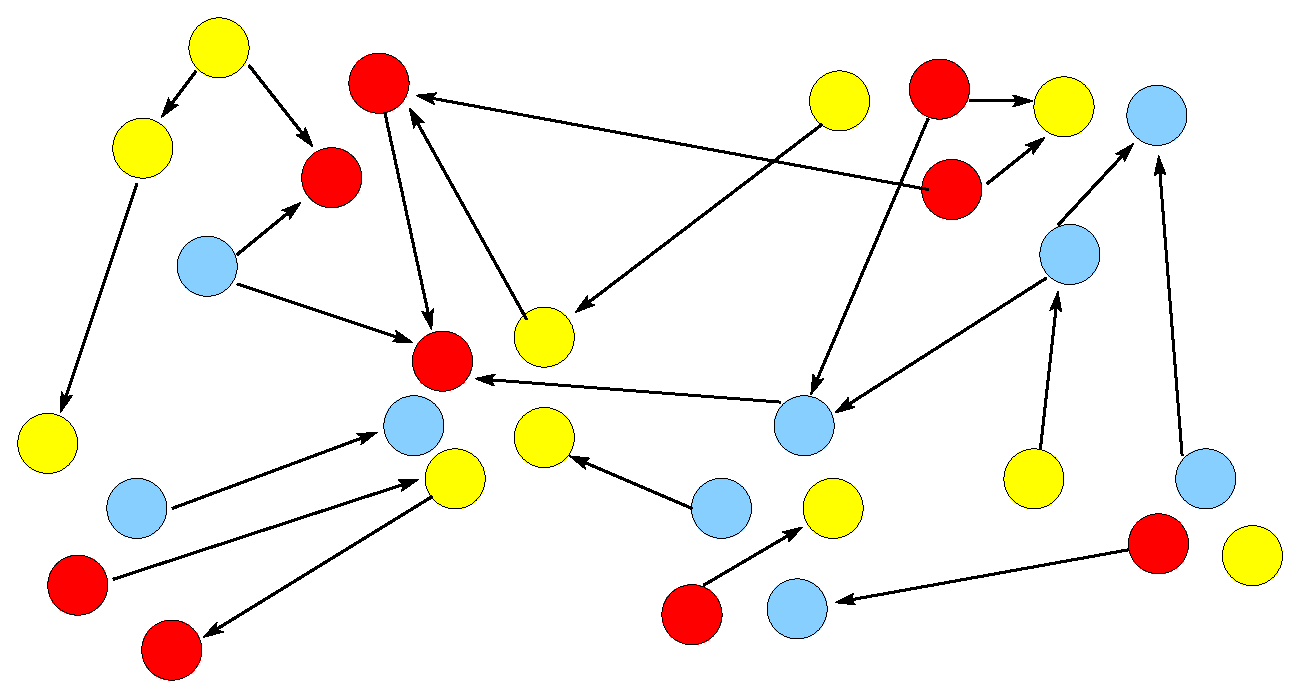
\includegraphics[width=0.45\linewidth]{gm.eps}  }
\caption{Subfigure example}
\end{figure}

\subsection{Equations}
$y=Cx$
\begin{equation}
	F(s) = \int_0^\infty e^{-st} f(t) dt
\end{equation}
the package 'align'
\begin{align}
    x    &= 2 \label{eq:x} \\
    y    &= 3 \label{eq:y} \\
    z    &= x \times y \nonumber \\
        &= p \label{eq:results}
\end{align}
\begin{itemize}
\item To not include an equation number, use \texttt{\nonumber} or \texttt{notag} 
\item Cross referencing can be done using \texttt{ref} or \texttt{eqref} together with \texttt{label}. For example, we refer to~\eqref{eq:x} that $x=2$.
\end{itemize}
the package 'eqnarray' is another environment to arrange equations into array format.
\begin{eqnarray}
\dot{x} &=& Ax + Bu \\
y &=& Cx+Du
\end{eqnarray}
If we want to align all equations into center use the package 'gather'.
\begin{gather}
y = \sum_{n=0}^100 0.5^n + \sin(2\pi n t) + \lim_{n \rightarrow \infty} \frac{\log n}{n} \\
z = \lim_{t \rightarrow \infty} e^{-st} g(t) 
\end{gather}

\subsection{References}
Reference formats are different from reference types. We commonly use the IEEE format, found in 

\url{https://ieee-dataport.org/sites/default/files/analysis/27/IEEE Citation Guidelines.pdf}

Use BibTex to generate reference list in the document. You will need a list of reference in the format of \texttt{file.bib} containing reference details, which can be exported easily using Google Scholar. When to refer to a paper, use \texttt{cite}. For example, the concept about system identification can be read from~\cite{SoS:89}. test \cite{CPM:89},\citep{CaA:15}, \cite{GrB:08b},\citep{JiY:09}

\bibliography{ref}
\bibliographystyle{ieeetr}

\section{Appendices}

\subsection{Appendix A}

\subsection{Appendix B}

\end{document}